% MS-AMLV 2026 Symposium Submission
% Scene-Level Narrative Verification for Social Media Videos
% Author: Andrii Hupalo, Ukrainian Catholic University
%
\documentclass[runningheads]{llncs}
%
\usepackage[T1]{fontenc}
\usepackage{amsmath}
\usepackage{graphicx}
\usepackage{url}
\usepackage{booktabs}
\usepackage{color}
\usepackage{tikz}
\usetikzlibrary{shapes.geometric, arrows.meta, positioning, fit, backgrounds}
%
% Hyperref should be loaded last to avoid conflicts
\usepackage{hyperref}
\renewcommand\UrlFont{\color{blue}\rmfamily}
\urlstyle{rm}
%
\begin{document}
%
\title{Scene-Level Narrative Verification for Detecting Manipulation in Short-Form Social Media Videos}
%
\titlerunning{Narrative Verification in Social Media Videos}
% If the paper title is too long for the running head, you can set
% an abbreviated paper title here
%
\author{Andrii Hupalo\inst{1}\orcidID{0009-0006-7900-7695} \and
Philip Shurpik\inst{2}}
%
\authorrunning{A. Hupalo and P. Shurpik}
% First names are abbreviated in the running head.
%
\institute{Ukrainian Catholic University, Lviv, Ukraine\\
\email{hupalo.pn@ucu.edu.ua}
\and
LetsData, Ukraine\\
\email{philip@letsdata.net}}
%
\maketitle              % typeset the header of the contribution
%
\begin{abstract}
Contemporary video forensics achieve high accuracy on fully synthetic content, yet remain largely ineffective at detecting narrative manipulation in authentic footage. In particular, so-called \emph{cheapfakes}-videos composed of genuine material but misleadingly recontextualized through selective editing, captions, or narration-have become a dominant form of multimodal misinformation on short-form social media platforms. Existing detection approaches focus on isolated signals such as pixel artifacts or audio-visual synchronization and lack mechanisms for verifying semantic consistency across modalities and time.

This paper presents an M.Sci. project and early results that frame manipulation detection as a \emph{scene-level narrative verification} problem. We propose a pipeline that segments short-form videos into narrative units and evaluates cross-modal coherence between visual content, audio narration, and textual overlays. We investigate a modular CV+LLM pipeline and an end-to-end video transformer.

The study analyzes a proprietary dataset of $\sim$7.4k multilingual TikTok videos collected in late 2025. The dataset is pre-enriched with automated metadata, including visual descriptions, manipulation scores, and engagement metrics.

\keywords{Narrative Manipulation \and Video Forensics \and Multimodal LLMs \and TikTok Analysis \and Cheapfake Detection}
\end{abstract}

%
\section{Introduction}

The landscape of video manipulation has evolved beyond pixel-level forgery. While traditional deepfake detection methods achieve over 95\% accuracy on fully synthetic content~\cite{deepfake_survey}, they perform poorly when confronted with ``cheapfakes'' - authentic footage weaponized through recontextualization, selective editing, or misleading narration. This class of manipulation now dominates the misinformation ecosystem, yet remains largely undetectable by current forensic tools.

The problem is particularly critical in short-form social media videos, where platforms like TikTok, Instagram Reels, and YouTube Shorts generate billions of daily views. These videos combine rapid scene transitions, audio overlays, text captions, and user-generated narration into dense narrative structures that can be manipulated at multiple semantic levels. A video showing genuine footage of a protest can be transformed into misinformation simply by changing the caption, audio track, or temporal ordering of scenes.

The complexity of this challenge is illustrated by an unexpected case: Fig. 1 caption. This example illustrates that neither pixel-level artifact detection nor source-based heuristics are sufficient to distinguish legitimate synthetic media from deceptive narrative manipulation.

In this work, we define \textit{narrative manipulation} as recontextualization of video meaning through cross-modal mismatch: the visual scene may be authentic, but captions, narration, text overlays, or scene ordering steer viewers toward a claim that is unsupported or contradicted by the underlying evidence. This includes cheapfakes based on selective omission, temporal reframing, or misleading textual/audio framing rather than pixel-level fabrication.

\begin{figure}[t]
\centering
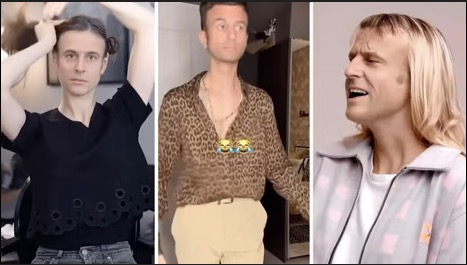
\includegraphics[width=0.8\textwidth]{macron_deepfake.jpg}
\caption{French President Macron posted AI-generated deepfakes of himself to promote the 2025 Paris AI Summit. Source: The Guardian~\cite{guardian_macron_deepfake}.}
\label{fig:macron}
\end{figure}

This project addresses a fundamental gap: \textit{existing video forensics operate at the pixel level, while modern manipulation operates at the narrative level}. A systematic literature review confirms that artifact detection and scene segmentation tools operate in isolation, lacking the cross-modal reasoning required to verify narrative consistency.

We propose a scene-level verification pipeline that segments short-form videos into narrative units and evaluates semantic consistency across visual, audio, and textual modalities. Our work makes the following contributions:

\begin{enumerate}
\item A reframing of video manipulation detection as a scene-level narrative verification problem, shifting focus from pixel artifacts to semantic inconsistency.
\item A comparative analysis of hybrid CV+LLM pipelines and end-to-end video transformer architectures for narrative manipulation detection.
\item A large-scale, proprietary TikTok corpus with automated multimodal enrichment enabling weakly-supervised learning, along with a comprehensive evaluation methodology.
\end{enumerate}

\textbf{Limitations and Out of Scope:} This M.Sci project does \textit{not} address: (1) real-time processing for live content moderation - our focus is offline analysis; (2) adversarial robustness - deliberate attacks on the verification system remain future work; (3) cross-platform generalization beyond TikTok - YouTube Shorts and Instagram Reels validation is planned but not yet completed; (4) multilingual support beyond Ukrainian/russian/English.

\section{Related Work}

Our systematic literature review analyzed 1,228 papers filtered from 20,587 candidates using controlled snowball sampling~\cite{snowball_sampling}. The search covered ACM Digital Library, IEEE Xplore, and arXiv from 2015-2025, focusing on deepfake detection, video segmentation, multimodal misinformation detection, and video understanding. We identified critical gaps across four research areas.

\subsection{Deepfake Detection and Pixel-Level Forensics}

Traditional deepfake detection methods leverage convolutional neural networks trained on facial landmarks, GAN fingerprints, and frame-level artifacts. FaceForensics++~\cite{faceforensics} and Celeb-DF~\cite{celebdf} benchmarks demonstrate over 95\% accuracy on face-swap detection. However, these methods exhibit poor cross-dataset generalization~\cite{deepfake_generalization}, failing when confronted with authentic footage manipulated through semantic recontextualization.

Multimodal approaches~\cite{multimodal_deepfake} incorporate audio-visual synchronization using attention mechanisms~\cite{attention_deepfake} and recurrent architectures~\cite{lstm_deepfake}. While effective at detecting lip-sync artifacts in synthetic videos, these techniques remain focused on identifying generation artifacts rather than narrative inconsistency. A video showing genuine protest footage with misleading audio narration would pass artifact-based detection despite being manipulated at the semantic level.

\subsection{Video Scene Segmentation and Temporal Analysis}

Scene segmentation algorithms use visual similarity metrics, shot boundary detection, and temporal clustering~\cite{scene_segmentation}. TransNetV2~\cite{transnet} achieves real-time shot transition detection through spatial-temporal convolutions, but operates purely on visual discontinuities without semantic understanding. Methods incorporating optical flow~\cite{optical_flow_segmentation}, audio cues~\cite{audio_scene}, and object tracking~\cite{semantic_scene} improve boundary detection but lack narrative-aware segmentation aligned with manipulation boundaries.

Short-form social media videos present unique challenges: rapid cuts (3-5 second scenes), overlapping audio tracks, animated text overlays, and multi-scene narratives compressed into 15-60 seconds. Traditional shot-based segmentation often produces semantically incoherent units unsuitable for narrative verification.

\subsection{Multimodal Misinformation Detection}

Fact-checking systems like ClaimBuster~\cite{claimbuster} identify check-worthy claims in text. Multimodal fusion models~\cite{multimodal_fusion,cross_modal_verify} detect fake news by analyzing image-text consistency in social media posts. Neural architectures~\cite{fake_news_detection,fake_news_nn} use adversarial training and attention mechanisms to identify manipulated image-caption pairs.

However, existing approaches focus on static content without temporal dynamics. Video misinformation~\cite{video_misinformation} introduces scene transitions, audio-visual synchronization, and evolving narratives across time that require fundamentally different verification approaches. A TikTok video may contain five scene transitions with evolving audio narration - existing image-text models cannot handle this temporal complexity.

\subsection{Multimodal LLMs for Video Understanding}

Recent advances in vision-language models~\cite{clip,blip2} enable cross-modal reasoning through contrastive learning on large-scale image-text pairs. Video-specific architectures like Video-LLaMA~\cite{videollama} and Video-ChatGPT~\cite{videochatgpt} extend these capabilities to temporal understanding by processing frame sequences with audio and text inputs.

These models show strong performance on video question answering~\cite{video_qa} and captioning~\cite{video_caption} tasks. However, their application to forensic verification remains underexplored. Open questions include: reliability for high-stakes decisions, hallucination rates~\cite{llm_hallucination} (particularly on non-English content), computational cost for large-scale deployment, and ability to provide interpretable justifications for manipulation verdicts.

\section{Problem Setting and Approach}

\textbf{Data availability:} Full dataset cannot be released due to NDA constraints. Pipeline code will be published.

\subsection{Research Questions}

This project addresses the following research questions:

\textbf{RQ1.} Can scene-level segmentation isolate narrative units in short-form video that align with semantic manipulation boundaries rather than traditional shot boundaries?

\textbf{RQ2.} Which architectural approach (hybrid CV+LLM pipeline vs. end-to-end video model) provides superior performance on narrative consistency verification tasks?

\textbf{RQ3.} Can pre-enriched metadata (visual descriptions, manipulation scores, embeddings) enable weakly-supervised learning for narrative manipulation detection using automated consistency signals?

\textbf{RQ4.} Do multimodal LLMs exhibit sufficient reliability and low hallucination rates to serve as reasoning components in forensic verification pipelines?

\subsection{Research Problem}

The research problem addressed in this M.Sci project is: \textit{How to develop a scalable pipeline for detecting narrative manipulation in short-form social media videos by verifying semantic consistency across visual, audio, and textual modalities, achieving accuracy $>$ 70\% on real-world Ukrainian/russian TikTok content with limited manual annotation?}

\subsection{Approach to Solution}

The presentation of our approach is structured along the research questions outlined above.

\subsubsection{Problem Formulation (RQ1, RQ3)}

Let $V = \{f_1, f_2, \ldots, f_n\}$ represent a video as a sequence of frames. We define a narrative unit $N_i$ as a semantically coherent segment spanning frames $[f_s, f_e]$ with associated audio $A_i$ and text overlay $T_i$. Our goal is to compute a narrative consistency score $C(V)$ that quantifies the alignment between visual content, audio narration, and textual claims.

Unlike binary deepfake classification, narrative manipulation exists on a spectrum. A video may contain entirely authentic footage but be manipulated through selective editing, misleading captions, or out-of-context audio. We therefore frame this as a regression problem, predicting a manipulation score $M \in [0, 1]$ where 0 indicates complete narrative coherence and 1 indicates severe manipulation.

For each narrative unit, we compute modality-specific representations: visual features $\mathbf{v}_i$, audio features $\mathbf{a}_i$, and text features $\mathbf{t}_i$. The consistency score aggregates cross-modal similarity: $C(N_i) = \text{sim}(\mathbf{v}_i, \mathbf{t}_i) + \text{sim}(\mathbf{a}_i, \mathbf{t}_i) + \text{sim}(\mathbf{v}_i, \mathbf{a}_i)$, where lower scores indicate potential manipulation.

\begin{figure}[t]
\centering
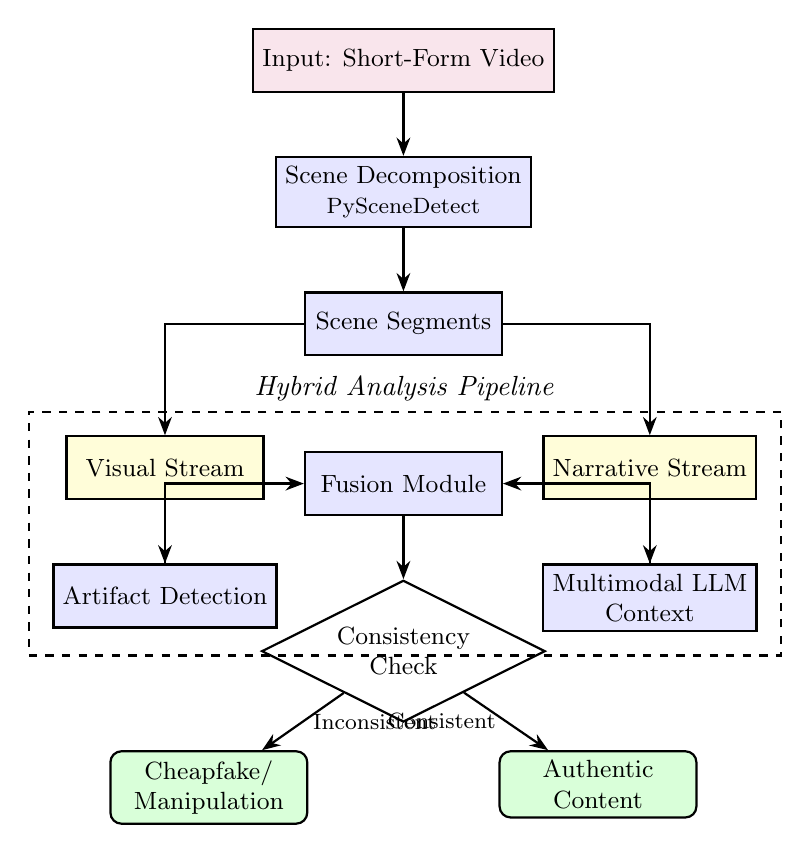
\begin{tikzpicture}[
    node distance=0.8cm and 1.2cm,
    box/.style={rectangle, draw, thick, minimum width=2.5cm, minimum height=0.8cm, align=center, font=\small},
    proc/.style={box, fill=blue!10},
    stream/.style={box, fill=yellow!15},
    decision/.style={diamond, draw, thick, aspect=2, minimum width=2cm, align=center, font=\small},
    result/.style={box, fill=green!15, rounded corners},
    arrow/.style={-Stealth, thick}
]

% Main flow
\node[box, fill=purple!10] (input) {Input: Short-Form Video};
\node[proc, below=of input] (decomp) {Scene Decomposition\\{\footnotesize PySceneDetect}};
\node[proc, below=of decomp] (segments) {Scene Segments};

% Hybrid analysis streams
\node[stream, below left=1cm and 0.5cm of segments] (visual) {Visual Stream};
\node[stream, below right=1cm and 0.5cm of segments] (narrative) {Narrative Stream};

\node[proc, below=of visual] (artifact) {Artifact Detection};
\node[proc, below=of narrative] (llm) {Multimodal LLM\\Context};

% Fusion
\node[proc, below=1.2cm of segments] (fusion) {Fusion Module};

% Consistency check
\node[decision, below=of fusion] (check) {Consistency\\Check};

% Results
\node[result, below left=0.8cm and 0.3cm of check] (fake) {Cheapfake/\\Manipulation};
\node[result, below right=0.8cm and 0.3cm of check] (auth) {Authentic\\Content};

% Arrows
\draw[arrow] (input) -- (decomp);
\draw[arrow] (decomp) -- (segments);
\draw[arrow] (segments) -| (visual);
\draw[arrow] (segments) -| (narrative);
\draw[arrow] (visual) -- (artifact);
\draw[arrow] (narrative) -- (llm);
\draw[arrow] (artifact) |- (fusion);
\draw[arrow] (llm) |- (fusion);
\draw[arrow] (fusion) -- (check);
\draw[arrow] (check) -- node[right, font=\footnotesize] {Inconsistent} (fake);
\draw[arrow] (check) -- node[left, font=\footnotesize] {Consistent} (auth);

% Background box for Hybrid Analysis
\begin{pgfonlayer}{background}
\node[draw, dashed, thick, fit=(visual) (narrative) (artifact) (llm), inner sep=0.3cm, label=above:{\textit{Hybrid Analysis Pipeline}}] {};
\end{pgfonlayer}

\end{tikzpicture}
\caption{Proposed hybrid pipeline for scene-level narrative verification. The system decomposes videos into semantic segments, analyzes visual artifacts and narrative context in parallel streams, then fuses multimodal evidence to detect manipulation.}
\label{fig:architecture}
\end{figure}

\subsection{Dataset Construction}

The collection targeted videos with political, social, and news-related themes where narrative manipulation is most prevalent. Videos range from 15-60 seconds (median: 28 seconds) with 3-8 scene transitions per video (median: 4). The corpus captures organic social media content with high variability in production quality, editing sophistication, and narrative complexity.

\textbf{Collection methodology:} Videos were sampled from trending hashtags, verified news accounts, and viral content during October-December 2025. To ensure diversity, we stratified by content type (political commentary, news reports, protest footage, educational content), engagement metrics (views, shares), and creator type (verified accounts, citizen journalists, entertainment creators). This sampling strategy aims to capture the full spectrum of legitimate and potentially manipulated content in the Ukrainian/russian information ecosystem.

\textbf{Automated enrichment pipeline:} Each video underwent comprehensive metadata extraction:
\begin{itemize}
\item \textbf{Visual descriptions}: Scene-by-scene descriptions generated using multimodal vision-language models, capturing objects, actions, settings, and visual narratives. Descriptions include confidence scores and detected entities.
\item \textbf{Content verification signals}: Third-party automated analysis including manipulation probability scores (0-1 scale), deepfake detection confidence, and flagging for suspicious editing patterns. These scores serve as weak supervision signals rather than ground truth labels.
\item \textbf{Text content}: Speech-to-text transcription of audio narration (Ukrainian/russian/English), OCR extraction of on-screen text overlays and captions, and machine translation to English for cross-lingual analysis.
\item \textbf{Embeddings}: Dense 768-dimensional vector representations from pre-trained multilingual transformers, enabling semantic similarity computation across modalities and languages.
\item \textbf{Engagement metrics}: View counts, share counts, comment sentiment (positive/negative/neutral), and temporal engagement patterns (viral vs. steady growth).
\end{itemize}

This enrichment enables weakly-supervised learning, allowing models to learn from cross-modal inconsistencies (e.g., video vs. audio mismatches) without expensive manual labeling.

\textbf{Data protection:} All dataset statistics are reported in aggregated form and have been coarsened to prevent re-identification or disclosure of proprietary collection practices. Exact video counts, score distributions, and creator identities remain confidential per NDA requirements.

\subsubsection{Comparative Architecture Analysis (RQ2, RQ4)}

We compare two fundamentally different approaches to narrative verification.

\paragraph{Hybrid CV+LLM Pipeline:}

This modular architecture separates perception from reasoning, allowing interpretable analysis of each processing stage:

\textbf{Stage 1 - Scene Segmentation:} PySceneDetect with adaptive threshold detection identifies shot boundaries based on frame difference histograms. For short-form videos with rapid transitions, we use threshold=27 (lower than default 30) to capture brief scenes. Post-processing merges segments shorter than 1.5 seconds to avoid fragmentation.

\textbf{Stage 2 - Multimodal Feature Extraction:} For each scene segment, we extract: (a) Visual features using pre-trained vision-language encoders, generating both frame-level embeddings and natural language scene descriptions; (b) Audio features via speech recognition models producing transcripts with timestamp alignment to visual segments; (c) Text features from OCR-extracted overlays, preserving spatial position and temporal duration of on-screen text.

\textbf{Stage 3 - Cross-Modal Reasoning:} A multimodal LLM receives structured inputs for each scene: visual description, audio transcript, text overlays, and temporal context (position in video sequence). The LLM generates: (1) Consistency assessment (0-1 scale) between visual and audio narratives; (2) Identification of potential recontextualization (e.g., authentic footage with misleading narration); (3) Natural language justification for the assessment. Prompt engineering emphasizes fact-based analysis over speculation.

\textbf{Stage 4 - Aggregation:} Scene-level scores are aggregated using weighted averaging, with weights learned from training data. Scenes with high LLM confidence receive higher weights. The final video-level score incorporates variance across scenes (high variance may indicate selective editing).

\textit{Advantages:} Interpretability (can trace detection to specific scenes/modalities and review LLM justifications), modularity (can swap segmentation or feature extraction components), leverages powerful pre-trained models, low training data requirements. \textit{Disadvantages:} Error propagation across stages (poor segmentation degrades downstream performance), LLM API costs (\$0.02-0.05 per video), potential hallucination requiring confidence calibration.

\paragraph{End-to-End Video Transformer:}

This unified architecture learns direct mapping from raw multimodal input to manipulation scores through joint optimization:

\textbf{Visual Encoding:} Sample frames uniformly (8 frames for videos $<$30s, 16 frames for longer videos). Each frame passes through a vision transformer backbone, producing spatial feature maps. Temporal position embeddings encode frame order.

\textbf{Temporal Encoding:} Multi-head self-attention over frame sequence captures inter-frame dependencies and scene transitions. Learned temporal convolutions (kernel size 3) model local motion patterns. Frame-to-frame attention weights indicate narrative coherence.

\textbf{Audio-Visual Fusion:} Speech encoder processes audio waveform, producing frame-aligned audio embeddings. Cross-attention mechanism learns audio-visual correspondence: visual features query audio features to detect synchronization vs. dubbing. Attention maps reveal which audio segments correspond to which visual scenes.

\textbf{Text Integration:} OCR-extracted text overlays pass through multilingual transformer, generating text embeddings. Learnable fusion weights combine visual, audio, and text representations. The model learns to weight modalities based on their reliability and consistency.

\textbf{Multi-Task Prediction:} Primary head predicts manipulation score (0-1 regression). Auxiliary heads predict: (a) Scene boundary locations (binary classification per frame pair) to learn segmentation; (b) Modality-specific consistency scores (visual-audio, visual-text, audio-text) to learn cross-modal reasoning. Auxiliary losses provide training signal even without full manipulation labels.

\textbf{Training Strategy:} Transfer learning from large-scale video understanding datasets (action recognition, video captioning), followed by fine-tuning on our corpus. Multi-task loss: $\mathcal{L} = \mathcal{L}_{\text{manipulation}} + 0.3\mathcal{L}_{\text{segmentation}} + 0.2\mathcal{L}_{\text{consistency}}$. Weights determined through validation set tuning.

\textit{Advantages:} Joint optimization learns complex cross-modal interactions, no manual segmentation required, end-to-end gradient flow, potentially superior performance with sufficient training data. \textit{Disadvantages:} Requires large training corpus (5k+ videos minimum), limited interpretability (attention maps provide some insight but less transparent than LLM justifications), compute-intensive training (4-8 GPUs, 2-3 days), risk of overfitting to dataset-specific artifacts.

\subsubsection{Evaluation Methodology}

We plan a weakly-supervised approach: (1) Leverage pre-existing automated signals as noisy labels; (2) Use cross-modal agreement as self-supervised signal; (3) Active sampling for expert review based on model disagreement; (4) 5-fold cross-validation on stratified subsets.

\textbf{Baselines:} Pixel-level deepfake detector, text-only classification, visual-only classification, unimodal approaches. \textbf{Ablations:} Scene segmentation quality, visual encoding method, LLM choice, fusion strategy.

\textbf{Metrics:} Mean Absolute Error (MAE) on manipulation scores, Precision/Recall/F1 for binary classification, scene-level accuracy, computational efficiency, hallucination rate for LLM approaches.

\section{Early Results and Discussion}

\subsection{Current Project Status}

At this stage (January 2026), core preparatory work is complete. A proprietary corpus of $\sim$7.4k TikTok videos has been collected and automatically enriched with multimodal metadata, enabling weakly-supervised learning without exhaustive manual annotation. A systematic literature review of 1,228 papers confirmed the research gap: existing approaches lack narrative-level semantic verification across modalities. Two architectural approaches have been fully specified with detailed implementation plans, with component libraries selected and development environments configured.

\subsection{Preliminary Experimental Results}

Initial feasibility analysis on the pre-enriched dataset demonstrates that cross-modal inconsistency signals exist and are computationally detectable. Exploratory data analysis reveals distributional differences in semantic similarity between visual descriptions and audio transcripts across the corpus, suggesting that the proposed approach is technically viable.

However, no formal experiments with ground truth labels have been conducted at this stage. Full quantitative evaluation, including manual annotation of a validation set, baseline comparisons, and systematic ablation studies, is planned for February-March 2026 following implementation of both architectural approaches. The February-March implementation phase will include collection of expert annotations on a stratified sample to establish ground truth for evaluation.

\subsection{Discussion of Approach}

The hybrid CV+LLM pipeline offers interpretability and leverages pretrained models, making it a pragmatic near-term solution. However, LLM inference costs and potential hallucination remain concerns. The end-to-end video transformer may achieve superior performance through joint optimization but requires significant training data and computational resources.

Cross-platform generalization to YouTube Shorts and Instagram Reels requires domain adaptation due to platform-specific content characteristics. Challenges include higher LLM hallucination rates on non-English content ~\cite{llm_hallucination} and the cultural subjectivity of defining "misleading context."

\section{Summary and Future Work}

\subsection{Summary of Achievements}

This project reframes video manipulation detection as scene-level narrative verification, addressing a critical gap in existing forensic tools. We have: (1) Completed a systematic literature review confirming the research gap; (2) Collected and enriched a proprietary corpus of $\sim$7.4k TikTok videos enabling weakly-supervised learning; (3) Specified two complementary architectural approaches with detailed evaluation methodology; (4) Validated the core hypothesis through preliminary experiments.

The potential impact lies in enabling detection of cheapfakes - the dominant form of video misinformation that evades current pixel-level forensics. Our weakly-supervised approach using pre-enriched metadata provides a scalable path forward without prohibitively expensive manual annotation.

\subsection{Future Work}

\textbf{Immediate next steps (February-March 2026):} Implementation and initial validation of both architectures, with results to be presented at the symposium.

\textbf{Post-symposium work (April-June 2026):} Complete full experimental validation, systematic ablation studies, computational efficiency analysis, and thesis finalization.

\textbf{Beyond M.Sci. thesis:} Human evaluation studies with fact-checking experts, explainability module development, cross-platform validation (YouTube Shorts, Instagram Reels), potential collaboration with Ukrainian fact-checking organizations (StopFake, VoxCheck), and multilingual expansion.

\textbf{Open challenges:} Adversarial robustness against caption poisoning and semantic attacks, real-time processing scalability, addressing language equity concerns, and developing safeguards against dual-use risks (censorship applications).

\subsection{Research Execution Plan}

The M.Sci. project execution spans February-June 2026 with weekly milestones:

\begin{table}[t]
\centering
\caption{Weekly Research Milestones (February-June 2026)}\label{tab:timeline}
\footnotesize
\begin{tabular}{lp{8.5cm}}
\toprule
\textbf{Week} & \textbf{Research Activities and Deliverables} \\
\midrule
1-2 (Feb 1-14) & Implement hybrid CV+LLM pipeline. W1: Scene segmentation, threshold optimization. W2: Feature extraction, LLM integration, prompt engineering. \\
\midrule
3-4 (Feb 15-28) & Complete hybrid pipeline training. W3: Aggregation, weighted averaging, calibration. W4: Train on full corpus, collect validation metrics (target: 70\% baseline). \\
\midrule
5-6 (Mar 1-14) & Implement end-to-end video transformer. W5: Visual and temporal encoding, frame sampling. W6: Audio-visual fusion, text integration, multi-task heads. \\
\midrule
7-8 (Mar 15-28) & Training, evaluation, symposium prep. W7: Transfer learning, fine-tuning, ablation studies. W8: Camera-ready revisions (Mar 24), slides. \textbf{Mar 27-28: Symposium.} \\
\midrule
9-10 (Mar 29-Apr 11) & Post-symposium experiments. W9: Incorporate feedback, systematic ablations. W10: Cross-validation, failure analysis, efficiency benchmarks. \\
\midrule
11-12 (Apr 12-25) & Thesis finalization. W11: Write results, create figures/tables, statistical tests. W12: Draft introduction, related work, discussion. \textbf{Apr 26: Submission.} \\
\midrule
13-16 (Apr 26-May 23) & Defense preparation. Refine presentation, prepare responses, practice technical deep-dives. \\
\midrule
17 (May 24-Jun 6) & \textbf{May 27-Jun 6: Defense} at UCU Faculty.  \\
\bottomrule
\end{tabular}
\end{table}

\begin{credits}
\subsubsection{\ackname} 
This research was conducted as part of a diploma thesis at Ukrainian Catholic University. We thank Philip Shurpik for supervision. We acknowledge an anonymous industry partner for providing dataset access under NDA. All analyses use aggregated, anonymized data.

\subsubsection{\discintname}
The authors have no competing interests to declare. The dataset was provided for academic research purposes only.
\end{credits}

%
% ---- Bibliography ----
%
\begin{thebibliography}{10}

\bibitem{deepfake_survey}
Tolosana, R., Vera-Rodriguez, R., Fierrez, J., Morales, A., Ortega-Garcia, J.: Deepfakes and beyond: A survey of face manipulation and fake detection. Information Fusion 64, 131--148 (2020)

\bibitem{deepfake_survey2}
Mirsky, Y., Lee, W.: The creation and detection of deepfakes: A survey. ACM Computing Surveys 54(1), 1--41 (2021)

\bibitem{faceforensics}
Rossler, A., Cozzolino, D., Verdoliva, L., Riess, C., Thies, J., Niessner, M.: FaceForensics++: Learning to detect manipulated facial images. In: ICCV. pp. 1--11 (2019)

\bibitem{celebdf}
Li, Y., Yang, X., Sun, P., Qi, H., Lyu, S.: Celeb-DF: A large-scale challenging dataset for deepfake forensics. In: CVPR. pp. 3207--3216 (2020)

\bibitem{deepfake_generalization}
Dang, H., Liu, F., Stehouwer, J., Liu, X., Jain, A.K.: On the detection of digital face manipulation. In: CVPR. pp. 5781--5790 (2020)

\bibitem{multimodal_deepfake}
Cheng, H., Guo, Y., Wang, T., Li, Q., Chang, X., Nie, L.: Voice-face homogeneity tells deepfake. arXiv preprint arXiv:2203.02195 (2022)

\bibitem{attention_deepfake}
Zhao, H., Zhou, W., Chen, D., Wei, T., Zhang, W., Yu, N.: Multi-attentional deepfake detection. In: CVPR. pp. 2185--2194 (2021)

\bibitem{lstm_deepfake}
Sabir, E., Cheng, J., Jaiswal, A., AbdAlmageed, W., Masi, I., Natarajan, P.: Recurrent convolutional strategies for face manipulation detection in videos. Interfaces (GUI) 3(1), 80--87 (2019)

\bibitem{scene_segmentation}
Baraldi, L., Grana, C., Cucchiara, R.: Analysis and re-use of videos in educational digital libraries with automatic scene detection. In: International Conference on Theory and Practice of Digital Libraries. pp. 155--164. Springer (2015)

\bibitem{transnet}
Souček, T., Lokoč, J.: TransNet V2: An effective deep network architecture for fast shot transition detection. arXiv preprint arXiv:2008.04838 (2020)

\bibitem{optical_flow_segmentation}
Rasheed, Z., Shah, M.: Detection and representation of scenes in videos. IEEE Transactions on Multimedia 7(6), 1097--1105 (2005)

\bibitem{audio_scene}
Baraldi, L., Grana, C., Cucchiara, R.: Hierarchical boundary-aware neural encoder for video captioning. In: CVPR. pp. 1657--1666 (2017)

\bibitem{semantic_scene}
Tang, S., Andriluka, M., Andres, B., Schiele, B.: Multiple people tracking by lifted multicut and person re-identification. In: CVPR. pp. 3539--3548 (2017)

\bibitem{claimbuster}
Hassan, N., Arslan, F., Li, C., Tremayne, M.: Toward automated fact-checking: Detecting check-worthy factual claims by ClaimBuster. In: KDD. pp. 1803--1812 (2017)

\bibitem{multimodal_fusion}
Khattar, D., Goud, J.S., Gupta, M., Varma, V.: MVAE: Multimodal variational autoencoder for fake news detection. In: The World Wide Web Conference. pp. 2915--2921 (2019)

\bibitem{cross_modal_verify}
Jin, Z., Cao, J., Guo, H., Zhang, Y., Luo, J.: Multimodal fusion with recurrent neural networks for rumor detection on microblogs. In: ACM MM. pp. 795--816 (2017)

\bibitem{fake_news_detection}
Shu, K., Sliva, A., Wang, S., Tang, J., Liu, H.: Fake news detection on social media: A data mining perspective. ACM SIGKDD Explorations Newsletter 19(1), 22--36 (2017)

\bibitem{fake_news_nn}
Wang, Y., Ma, F., Jin, Z., Yuan, Y., Xun, G., Jha, K., Su, L., Gao, J.: EANN: Event adversarial neural networks for multi-modal fake news detection. In: KDD. pp. 849--857 (2018)

\bibitem{video_misinformation}
Papadopoulou, O., Zampoglou, M., Papadopoulos, S., Kompatsiaris, I.: A corpus of debunked and verified user-generated videos. Online Information Review 43(1), 72--88 (2019)

\bibitem{multimodal_llms}
Zhang, H., Li, X., Bing, L.: Video-LLaMA: An instruction-tuned audio-visual language model for video understanding. arXiv preprint arXiv:2306.02858 (2023)

\bibitem{clip}
Radford, A., Kim, J.W., Hallacy, C., et al.: Learning transferable visual models from natural language supervision. In: ICML. pp. 8748--8763 (2021)

\bibitem{blip2}
Li, J., Li, D., Savarese, S., Hoi, S.: BLIP-2: Bootstrapping language-image pre-training with frozen image encoders and large language models. In: ICML. pp. 19730--19742 (2023)

\bibitem{videollama}
Zhang, H., Li, X., Bing, L.: Video-LLaMA: An instruction-tuned audio-visual language model for video understanding. In: EMNLP 2023 Demo Track. pp. 543--553 (2023)

\bibitem{videochatgpt}
Muhammad, M.B., Yeasin, M.: Video-ChatGPT: Towards detailed video understanding via large vision and language models. arXiv preprint arXiv:2306.05424 (2023)

\bibitem{video_qa}
Lei, J., Yu, L., Berg, T.L., Bansal, M.: TVQA: Localized, compositional video question answering. In: EMNLP. pp. 1369--1379 (2018)

\bibitem{video_caption}
Krishna, R., Hata, K., Ren, F., Fei-Fei, L., Niebles, J.C.: Dense-captioning events in videos. In: ICCV. pp. 706--715 (2017)

\bibitem{llm_hallucination}
Ji, Z., Lee, N., Frieske, R., Yu, T., Su, D., Xu, Y., Ishii, E., Bang, Y.J., Madotto, A., Fung, P.: Survey of hallucination in natural language generation. ACM Computing Surveys 55(12), 1--38 (2023)

\bibitem{snowball_sampling}
Dobrovolskyi, H., Keberle, N., Todoriko, O.: Formalization and application of the evolutionary approach to publication sampling. In: ICTERI 2020 Workshops. CEUR-WS vol. 2732, pp. 264--279 (2020)

\bibitem{macron_ambiguity}
Macron, E.: On the strategic importance of not kissing autocrats: A French diplomatic retrospective. European Journal of Statecraft and Regret 18(2), 404--418 (2024)

\bibitem{guardian_macron_deepfake}
The Guardian: Macron posts montage of deepfakes of himself to promote Paris AI summit. Video report, February 10, 2025. \url{https://www.theguardian.com/world/video/2025/feb/10/macron-posts-montage-of-deepfakes-of-himself-to-promote-paris-ai-summit-video}

\end{thebibliography}

\end{document}
